\documentclass{article}
\usepackage[utf8]{inputenc}
\usepackage{graphicx} 
\usepackage{amsmath} 
\setlength{\parindent}{4em}
\setlength{\parskip}{1em}
\renewcommand{\baselinestretch}{1.5}
\newcommand{\Tau}{\mathrm{T}}

\title{BLG 354E Homework - 4}
\author{Yunus Güngör }
\date{June 2018}

\begin{document}
	
	\maketitle
	
	\section{Answers}
	
	This homework only includes answers to given questions
	
	1)\par
		Reqired codes can be found at attached file.
		Results gotten:\par
		
	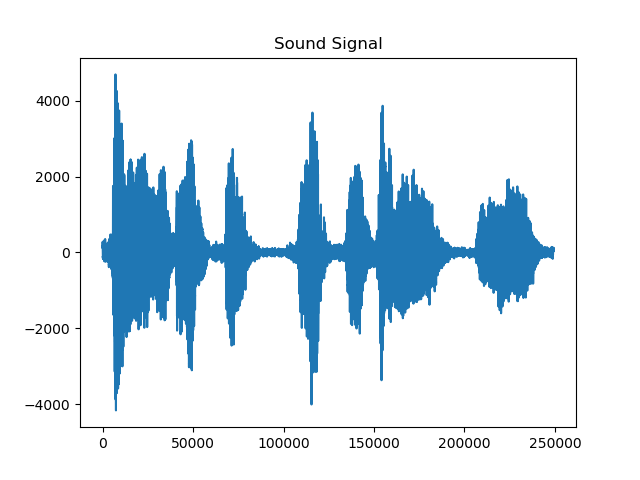
\includegraphics[scale=0.4]{sound_org}
	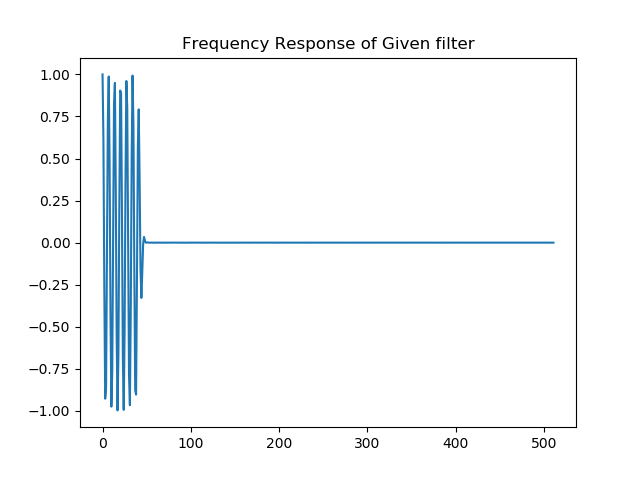
\includegraphics[scale=0.4]{freq_response}
	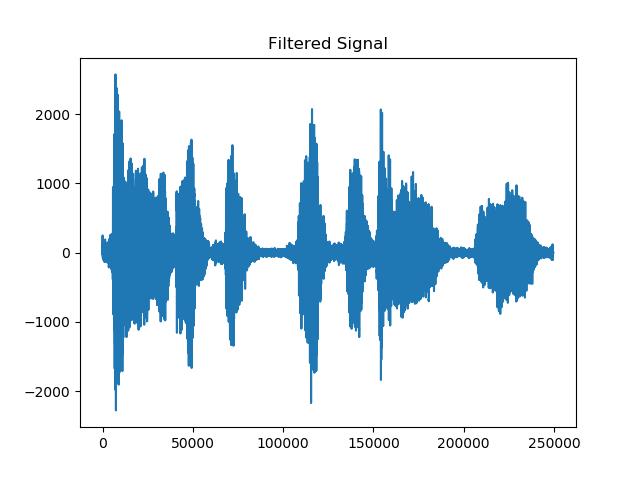
\includegraphics[scale=0.4]{filtered_signal}
	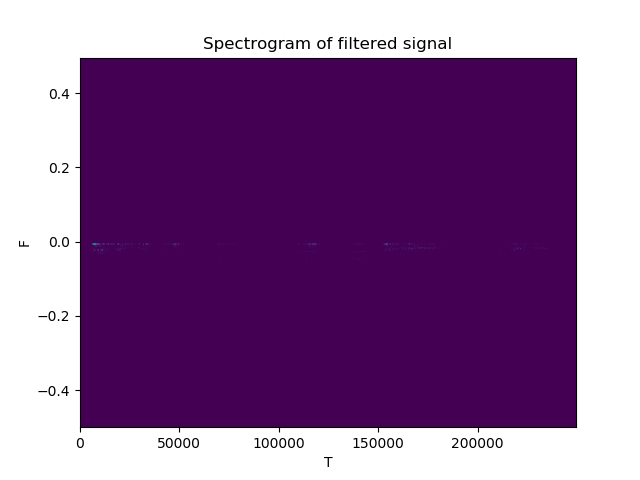
\includegraphics[scale=0.4]{spectogram}
	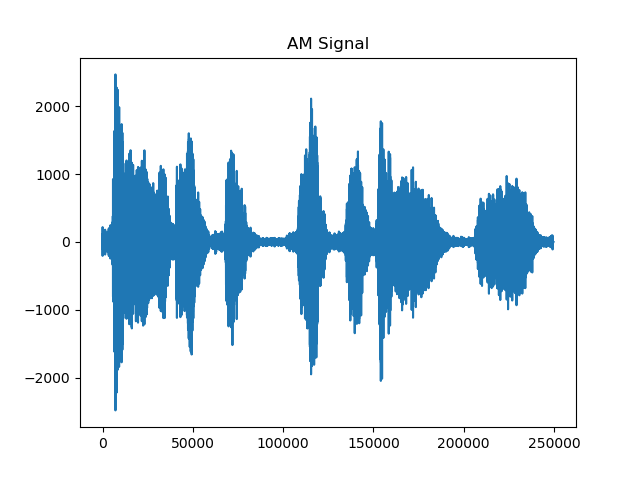
\includegraphics[scale=0.4]{AMSignal}
	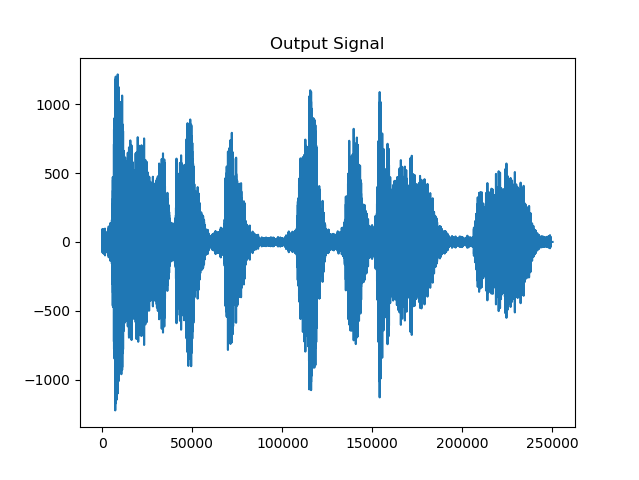
\includegraphics[scale=0.4]{output}
	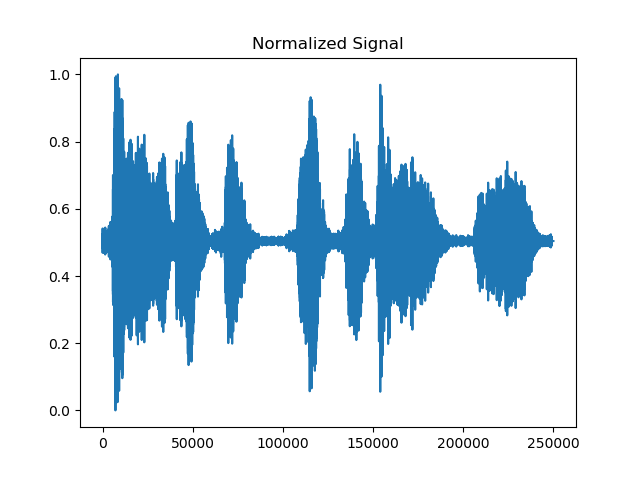
\includegraphics[scale=0.4]{normalized}
	\par 
	
	Demodulator output incresases, decreses and gets corrupt according to phase, and its zero for $\pi/2$.
	
	\par 
	
	When demodulator frequency has been set 10Hz higher than the modulator, signal becomes corrupted	
	
		  
	\par
\end{document}